\documentclass[letterpaper,10pt]{article}

\usepackage{enumitem}
\usepackage{titling}
\usepackage{listings}
\usepackage{url}
\usepackage{hyperref}
\usepackage{setspace}
\usepackage{subfig}
\usepackage{sectsty}
\usepackage{pdfpages}
\usepackage{colortbl}
\usepackage{multirow}
\usepackage{multicol}
\usepackage{relsize}
\usepackage{amsmath}
\usepackage{wasysym}
\usepackage{fancyvrb}
\usepackage[yyyymmdd]{datetime}
\usepackage{amsmath,amssymb,amsthm,graphicx,xspace}
\usepackage[titlenotnumbered,noend,noline]{algorithm2e}
\usepackage[compact]{titlesec}
\usepackage{XCharter}
\usepackage[T1]{fontenc}
\usepackage[scaled]{beramono}
\usepackage[normalem]{ulem}
\usepackage{booktabs}
\usepackage{tikz}
\usetikzlibrary{arrows,automata,shapes,trees,matrix,chains,scopes,positioning,calc}
\tikzstyle{block} = [rectangle, draw, fill=blue!20,
text width=2.5em, text centered, rounded corners, minimum height=2em]
\tikzstyle{bw} = [rectangle, draw, fill=blue!20,
text width=4em, text centered, rounded corners, minimum height=2em]

\definecolor{namerow}{cmyk}{.40,.40,.40,.40}
\definecolor{namecol}{cmyk}{.40,.40,.40,.40}
\renewcommand{\dateseparator}{-}

\let\LaTeXtitle\title
\renewcommand{\title}[1]{\LaTeXtitle{\textsf{#1}}}

\lstset{basicstyle=\footnotesize\ttfamily,breaklines=true}

\newcommand{\handout}[5]{
	\noindent
	\begin{center}
		\framebox{
			\vbox{
				\hbox to 5.78in { {\bf ECE 350: Real-Time Operating Systems } \hfill #2 }
				\vspace{4mm}
				\hbox to 5.78in { {\Large \hfill #4  \hfill} }
				\vspace{2mm}
				\hbox to 5.78in { {\em #3 \hfill \today} }
			}
		}
	\end{center}
	\vspace*{4mm}
}

\newcommand{\lecture}[3]{\handout{#1}{#2}{#3}{Lecture#1}}
\newcommand{\tuple}[1]{\ensuremath{\left\langle #1 \right\rangle}\xspace}

\newcommand{\Rplus}{\protect\hspace{-.1em}\protect\raisebox{.35ex}{\smaller{\smaller\textbf{+}}}}
\newcommand{\Cpp}{\mbox{C\Rplus\Rplus}\xspace}


\addtolength{\oddsidemargin}{-1.000in}
\addtolength{\evensidemargin}{-0.500in}
\addtolength{\textwidth}{2.0in}
\addtolength{\topmargin}{-1.000in}
\addtolength{\textheight}{1.75in}
\addtolength{\parskip}{\baselineskip}
\setlength{\parindent}{0in}
\renewcommand{\baselinestretch}{1.5}
\newcommand{\term}{Spring 2023}
\newcommand{\termnumeric}{1235}

\singlespace


\begin{document}

\lecture{ 17 --- Scheduling Algorithm Evaluation; UNIX \& Windows }{\term}{Jeff Zarnett}

\section*{Evaluating Scheduling Algorithms}

Although in some cases, like real-time scheduling, it is pretty obvious what algorithms we might want to use, in many cases, it isn't immediately obvious what scheduling routine makes the most sense or gives the best overall performance. This necessarily implies that there is a clear definition of best overall performance. We talked about some ten earlier and acknowledged they're not all equally important in a given system. Some are ignored altogether. That's okay.

Let's imagine, though, that you've made a decision of what's important in your system. However those are decided, we need to evaluate the algorithms we've discussed in terms of how well they achieve that goal. While it is possible to just have a theoretical discussion about it where we say we think $A$ is better than $B$ but worse than $C$, that's not a very scientific approach. What we'd like to do instead is gather some data and make the decision using it. Given that we don't have specific criteria for a system, this discussion will be restricted more to the idea of how to decide rather than walking through a specific decision. 

\paragraph{Deterministic Modelling.}

Deterministic modelling looks a lot like writing test scenarios for a lab project. The test scenario has some inputs and some outputs and then we can evaluate the outputs to check for both correctness and to assess the performance.  Why correctness? It's usually assumed that whatever algorithm that we are talking about is correct in its implementation, but evaluation of correctness in this context may mean things like processes do not starve.

Simple test cases will create all processes to run at the beginning and then put them into the ready queue. An example of a simple test case looks like this, where all five processes arrive at time 0 in this order~\cite{osc}:

\begin{center}
\begin{tabular}{c|r}
	\textbf{Process ID} & \textbf{Burst Time}\\ \hline
	1 & 10 \\
	2 & 29 \\
	3 & 3 \\
	4 & 7 \\
	5 & 12 \\
\end{tabular}
\end{center}

We can then run the target scheduling algorithm(s) and get some answers; the source shows that First-Come-First-Served results in an average wait time of 28 time units; Shortest-Job-First 13; Round-Robin with a timeslice of 10 time units has a waiting time of 23. In all cases, the total time of execution is the same -- there's no avoiding the work to be done -- but waiting times are different. In this example, the waiting time is the measure that we care about.

A more precise version of this evaluation would assign a penalty to the process switch. FCFS and SJF each have four process switches since processes do not get interrupted in the run. Round robin will have seven context switches, so it would be appropriate to say that the total execution time for the round robin evaluation is higher, although if context switches are very small as compared to the execution time, the tiny difference may be irrelevant.

Test cases that look more realistic will not have everything be statically initialized at the beginning and all tasks waiting. They will include tasks that arrive at the start, but also tasks that arrive after some time has passed, and may include periods where the idle task runs. They may also include other things, such as changing the priority of one or more threads as this will have an impact on the execution order of the various processes.

The nice thing about the deterministic modelling approach is that the tests are reproducible and produce consistent results on every run. Therefore, swapping or tweaking the algorithm under test and re-running the tests will make it pretty easy to identify the impact of the change (if any) that was made. 


\paragraph{Queueing Theory.}
Deterministic approaches are somewhat limited because the real behaviour of most systems looks very different from how the deterministic approach models it. Rather than a nice model of the world where things always happen in a fixed way, real systems have a lot of randomness in them: the time when a user requests something is, from the point of view of the computer, not really predictable. 

Yes, it may be the case that most people log in to a server at the start of their workday, but everyone's start of the workday is a little bit different, even if everyone is supposed to start at 09:00. Some people will be there a bit earlier, someone might be late because there's a crash on the highway, etc, or because a colleague stopped by their desk before they entered their username and password...  A model with some randomness built in might actually better reflect what happens... But not total randomness, because perhaps there are indeed some patterns like log-ins take place at the start of the day but not in the middle of the night.

That leads us to queueing theory! It is, as the saying goes, literally the theory of queues. What makes queues appear, how will they behave, and how do we make them go away? It does actually have the kind of modelling that we're looking for where we can treat arrivals of new things to do as random, and also have some sort of mathematical distribution for how long tasks execute. Given these models of what are called arrivals and departures we could then do some calculations around things like how busy the system is and how long processes have to wait.

The basic problem with queueing theory analysis is that it is mathematically complex and not suitable for every kind of scheduling algorithm; it also tends to force modelling things like request arrival times in ways that are easier to implement but not necessarily accurate~\cite{osc}.

Okay, queuing theory is too advanced for this course and we'll have to save it for a future one. It typically shows up as a graduate-level topic, but somehow, hints of it find their way into fourth year courses here and there.

\paragraph{Simulations and Emulation.}
Whatever modelling approach we choose, deterministic or statistical, we would get more accurate evaluations of the system by running a simulation. The simulation, if designed appropriately, will account for more things like clock interrupts and context switch times.

It's possible to do an all-software simulation, in which you just write some code and it runs as a regular process inside an existing operating system. The simulation has time steps and at each time step, the state of the system is updated as if certain things happened: the clock advances, timer interrupt runs, context switch takes place, etc. The simulation is only as accurate as you make it and there are a lot of things that might be difficult to simulate accurately (e.g., how often is there a cache miss?). It's difficult to make a simulation, but of course, it does not have to be perfect, just better than the alternatives.

Deciding what test scenarios you'd like to simulate is similar to the question about what test cases you want to execute in deterministic modelling. One possibility is the idea of traces~\cite{osc}: the basic idea is to record some actual executions on the system and use that as the basis for the test scenarios you'd like to run.

If you're writing code for another platform (e.g., an embedded system), that platform may come with an emulator which would be an even better place to evaluate the scheduling algorithm. The emulator is much slower than just running the simulation as a process inside another operating system, but it does give a much better understanding of how the system will actually perform since the emulator will have proper implementations of things like hardware and timer interrupts. And perhaps most importantly: you don't have to write the emulator; just use the existing one!

\paragraph{And then the real world...}
Simulations can only tell us so much about the actual performance of a scheduling algorithm, just because the simulation is always based on certain assumptions around user behaviour, external factors (network, etc), and the hardware that the user has. A general purpose operating system needs to work at an acceptable level on many different hardware configurations. 

And on that subject, well, we should take some time to consider the scheduling algorithms actually used in commercial desktop and server operating systems. Specifically, the traditional UNIX, Windows, and modern Linux scheduling approaches. I'm by no means saying that any of these operating systems have everything right and their form of scheduling is the optimal or ideal for the target use case, but if their choices were awful then user/customer pressure would surely force a change...

\section*{Commercial OS Scheduling Algorithms}

In this section we will examine how real commercial operating systems schedule their processes and threads. We will examine UNIX, Windows, and finally, Linux scheduling. We will see what approaches are used and what is interesting or novel about them. Truth be told, the traditional UNIX approach is dated, but it's worth talking about because a lot of the evolution of scheduling in Linux is based on overcoming the shortcomings of the traditional scheduler approach.

\subsection*{Traditional UNIX}

The traditional UNIX scheduling is really ancient; as in System V R3 and BSD 4.3. It was replaced in SVR4 (which had some real-time support). The information about the traditional UNIX scheduler comes primarily from~\cite{osi}.

The routine is a multilevel feedback system using Round Robin within each of the priority queues. Time slicing is implemented and the default time slice is a (very long) 1 second. So if a process does not block or complete within 1~s, then it will be preempted. Priority is based on the process type as well as the execution history.

Processor utilization for a process $j$ is calculated for an interval $i$ by the following formula:

\begin{center}
$CPU_{j}(i) = \dfrac{CPU_{j}(i - 1)}{2}$
\end{center}

And the priority is for process $j$ at interval $i$ is calculated by the formula:

\begin{center}
$P_{j}(i) = B_{j} + \dfrac{CPU_{j}}{2} + N_{j}$
\end{center}

where $B_{j}$ is the base priority of process $j$ and $N_{j}$ is the ``nice'' value of process $j$. The ``nice'' value is a UNIX way to allow a user to voluntarily reduce the priority of a process to be ``nice'' to other users (but honestly, who uses this?)~\cite{mos}. Actually, the answer to that question is: system administrators. An admin can ``re-nice'' a process and make it somewhat nicer than it would otherwise be.

The $CPU$ and $N$ components of the equation are restricted to prevent a process from migrating outside of its assigned category. A process is assigned to a given category based on what kind of process it is. To put it in simple terms, the OS puts its own needs first and tries to make the best use of resources it can. From highest to lowest priority, the categories are:

\begin{enumerate}
	\item Swapper (move processes to and from disk)
	\item Block I/O device control (e.g., disk)
	\item File manipulation
	\item Character I/O device control (e.g., keyboard)
	\item User processes
\end{enumerate}

Yes, unfortunately, user processes get piled at the bottom of the list. The use of the hierarchy should provide for efficient use of I/O devices and tends to penalize processor-bound processes at the expense of I/O bound processes. This is beneficial, because CPU-bound processes should be able to carry on executing when an I/O-bound process waits for the I/O operation to complete, but when an I/O operation is finished, we would like to start the next I/O operation so the I/O device is not waiting. This strategy is reasonably effective for a general-purpose, time-sharing operating system.

\paragraph{Upgrading to SRV4.}
In UNIX SRV4 the system for a complete overhaul, trying to give the highest priority to ``real-time'' processes, then kernel processes, and then user-mode preferences; its two big differences are (1) more priority levels -- 160 broken down into three types -- and (2) preemption points~\cite{osi}. 

Such preemption points are needed, because the original versions of the UNIX kernel were themselves not well-suited to preemption because it was not expected in the design that the kernel's execution could itself be preempted at any time. So preemption points are placed in the code where it would be okay for the kernel to stop execution and do another operation. In practice, this means that all kernel data structures are updated, or there are appropriate locks that would prevent concurrent modification and prevent race conditions~\cite{osi}. 

\paragraph{FreeBSD.}
BSD, the Berkeley Software Distribution, is another form of UNIX, and FreeBSD is one of its descendants. FreedBSD has a scheduling process that's quite similar to that of SRV4. There are more priority levels than SRV4 -- 256 rather than 160 -- and they are subdivided into five categories rather than just three. This implementation is intended to support multiprocessor systems better than the traditional UNIX approaches.

What's new and interesting here is the interactivity scoring mechanism. Interactivity score is intended to identify which threads are user-interactive and which ones are CPU-intensive. Threads that are user-interactive should get a higher priority to run; in this system, lower numbers equal higher priority. Interactivity is judged based on how much the thread in question gets blocked: if it's waiting for the user or network or similar, then it would be considered interactive.

The calculation looks like this~\cite{osi}: We'll define the maximum interactivity score as $m$, the runtime of the thread as $r$ and the sleep time of the thread as $s$. For threads that have more sleep time than run time, the interactivity score is calculated as $(\dfrac{m}{2})(\dfrac{r}{s})$ and for those that have more run time than sleep time:
  $(\dfrac{m}{2})(1 + \dfrac{r}{s})$. 
  
This system ensures that threads that sleep more than they run are always in the lower half, and threads that run more than they sleep are in the upper half of their priority bands. The mechanism is a little bit crude -- interactivity is a bit more complex than just whether the threads get blocked. One might expect that the solution is something like whether the program interacts with the console or UI fields, but users are good at gaming the system like this and doing unnecessary writes to the console to make the program appear more interactive than it is. So a crude method provides less reward for gaming the system, so to speak.

We've already discussed in some detail how thread affinity works and load-balancing across the different CPUs in the system. The FreeBSD scheduler uses both pull and push mechanisms to move threads to cores that are otherwise idle. The pull mechanism is simple enough: when a CPU has no work to do, it sets a bit in a bit mask to indicate that it's idle, and if a new thread is about to be added to a queue, the assignment mechanism checks for processors that are idle and sends it to them. The push migration is accomplished by the short-term scheduler twice per second and looks at the highest- and lowest-loaded processors and equalizes their run queues~\cite{osi}. 

\subsection*{Windows}

Windows schedules threads using a priority-based, preemptive scheduling algorithm, ensuring that the highest priority thread runs. The official name for the selection routine is the \textit{dispatcher}. A thread will run until it is preempted, blocks, terminates, or until its time slice expires. If a higher priority thread is unblocked, it will preempt a lower priority thread. Windows has 32 different priority levels, the regular (priority 1 to 15) and real-time classes (16 to 31). A memory management task runs at priority 0. The dispatcher maintains a queue for each of the scheduling priorities and goes through them from highest to lowest (yes, in Windows, higher numbers are higher priorities) until it finds something to do (and if there is nothing else currently ready, the System Idle Process will ``run'')~\cite{osc}.

There are six priority classes you can set a process to via Task Manager, from highest to lowest:
\begin{enumerate}
	\item Realtime
	\item High
	\item Above Normal
	\item Normal
	\item Below Normal
	\item Low
\end{enumerate}

A process is usually in the Normal class. Within that class there are some more relative priorities. Unless it is in the real-time category, the relative priority can change. The details are summarized in the table below:

\begin{center}
	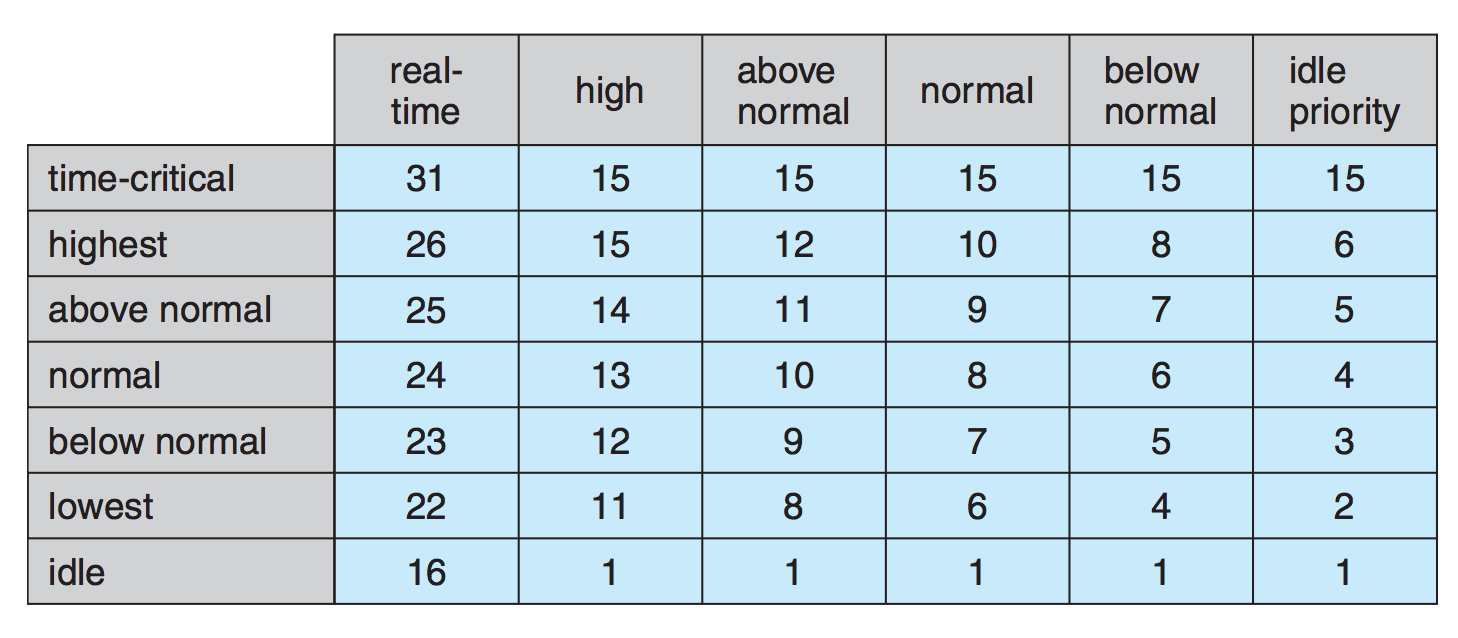
\includegraphics[width=0.7\textwidth]{images/windows-thread-priorities.png}\\
	Windows thread priorities~\cite{osc}.
\end{center}

If a process reaches the end of a time slice, the thread is interrupted. If it is not in the real-time category, its priority will be lowered, to a minimum of the base priority of each class. When a process that was blocked on something (e.g., a wait or I/O) is unblocked, its priority is temporarily boosted (unless it is real-time, in which case it cannot be boosted). The amount of the boost depends on what the event was: a process that was waiting for keyboard input gets a bigger boost than one that was waiting for a disk operation, for example~\cite{osc}. 

Windows also includes a little mechanism to make sure that a process does not starve; processes that have a low priority can temporarily get a boost to a priority of 15 to make sure that they get a chance to run and also to mitigate the impact of a potential priority inversion scenario~\cite{osi}.

The operating system also gives a priority to whatever process is running in the selected foreground window. This is different from foreground vs. background processes as discussed earlier, because the definition of a foreground process was one that was user-interactive. Here, the distinction is which of the user-interactive processes is currently ``on top'' in the UI. Not only does this process get a priority boost, but it also gets longer time slices. This can be disabled, if so desired, but it really highlights the different heritages of Windows and UNIX. UNIX was originally a time-sharing system with multiple users and lots of processes; Windows was originally a single-user desktop operating system doing one or maybe a few things at a time.


\bibliographystyle{alphaurl}
\bibliography{350}


\end{document}